% Schematic of the full second-order pipeline with the hybrid split of SR.
% Covers the distributional case (SR not integrable on the worldline). Compile with pdflatex.
\documentclass[tikz,border=4pt]{standalone}
\usepackage[T1]{fontenc}
\usepackage{lmodern}
\usepackage{amsmath,amssymb}
\usetikzlibrary{arrows.meta,decorations.pathreplacing,calc}
\newcommand{\PP}{\Phi^{\rm P}}
\newcommand{\Pres}{\Phi^{\rm res}}
\begin{document}
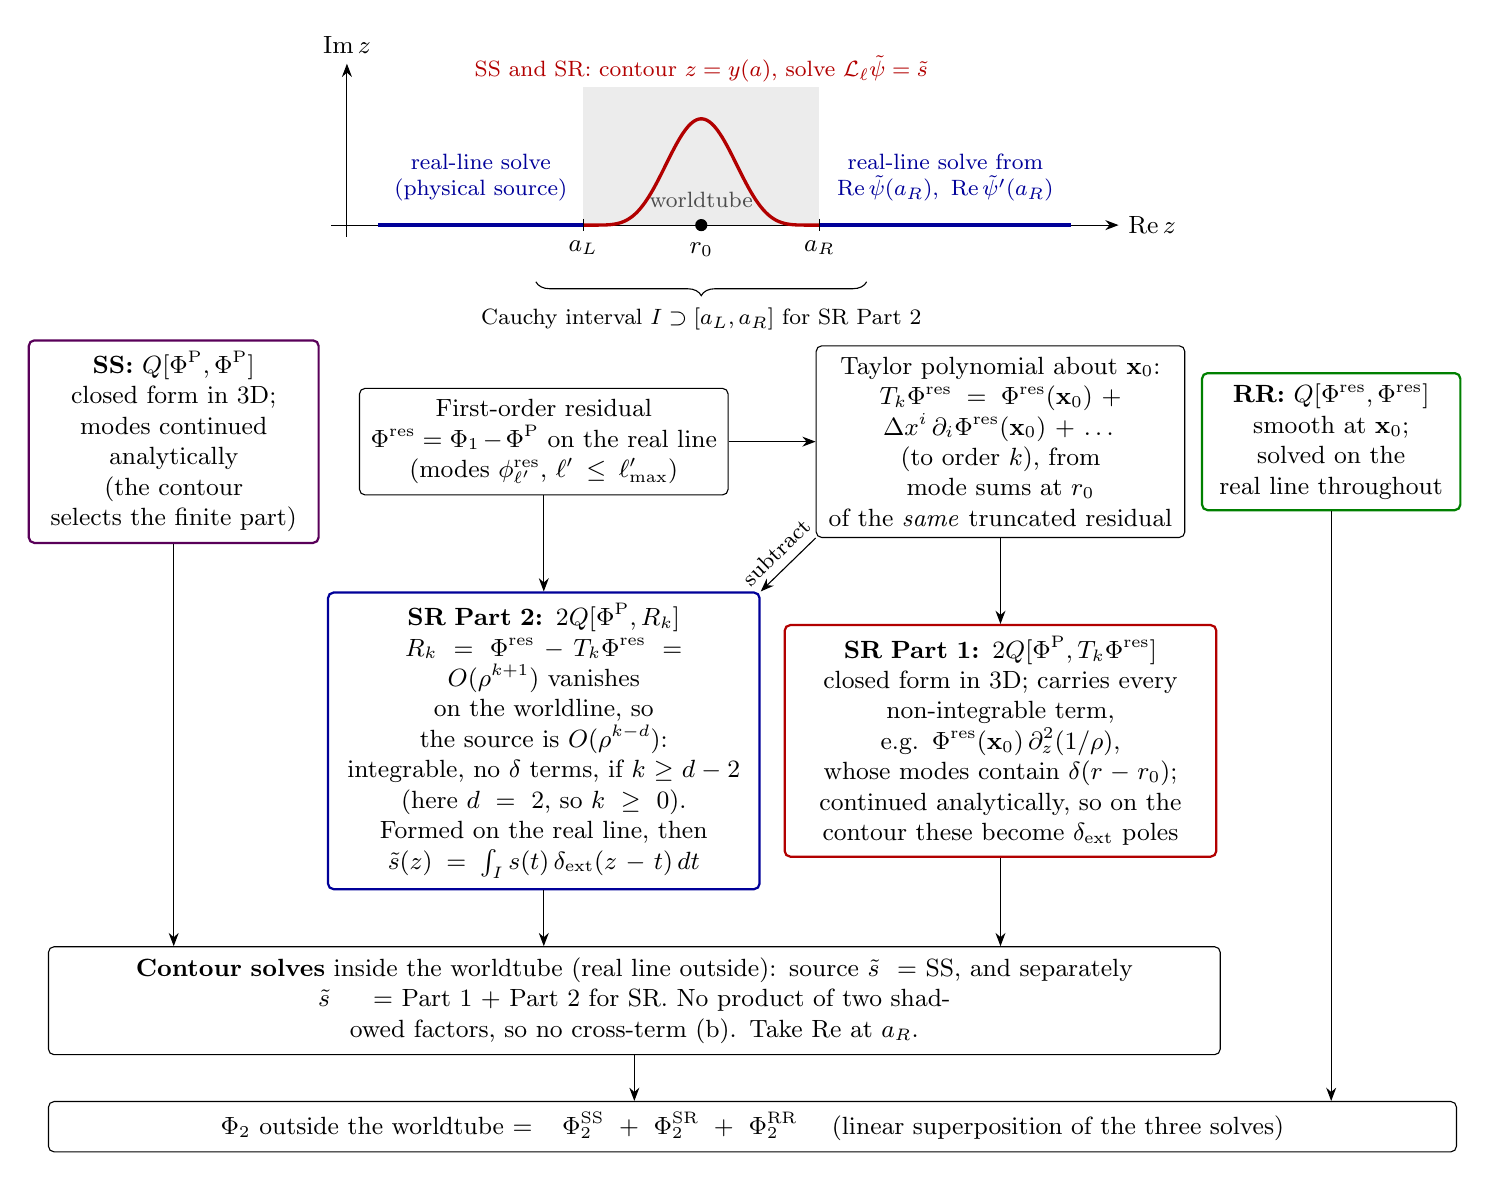
\begin{tikzpicture}[>=Stealth, font=\small,
  box/.style={draw, rounded corners=2pt, align=center, inner sep=4pt, text width=#1, fill=white},
  box/.default=4cm,
  note/.style={draw=gray!60, dashed, rounded corners=2pt, align=left, inner sep=4pt, fill=gray!6, font=\footnotesize}]

% ---------- complex r-plane ----------
\begin{scope}[xshift=3.6cm]
\fill[gray!15] (3.5,0) rectangle (6.5,1.75);
\node[gray!60!black, font=\footnotesize] at (5,0.32) {worldtube};
\draw[->] (0.3,0) -- (10.3,0) node[right] {$\operatorname{Re} z$};
\draw[->] (0.5,-0.15) -- (0.5,2.05) node[above] {$\operatorname{Im} z$};
\draw[very thick, blue!60!black] (0.9,0) -- (3.5,0);
\draw[very thick, blue!60!black] (6.5,0) -- (9.7,0);
\draw[very thick, red!70!black, domain=3.5:6.5, samples=120, smooth]
  plot (\x, {1.35*(1-((\x-5)/1.5)^2)^6});
\fill (5,0) circle (2.2pt);
\node[below=3pt] at (5,0) {$r_0$};
\draw (3.5,0.08) -- (3.5,-0.08) node[below] {$a_L$};
\draw (6.5,0.08) -- (6.5,-0.08) node[below] {$a_R$};
\draw[decorate, decoration={brace, mirror, amplitude=5pt}]
  (2.9,-0.72) -- (7.1,-0.72) node[midway, below=6pt, font=\footnotesize]
  {Cauchy interval $I\supset[a_L,a_R]$ for SR Part 2};
\node[blue!60!black, align=center, font=\footnotesize] at (2.2,0.6)
  {real-line solve\\(physical source)};
\node[blue!60!black, align=center, font=\footnotesize] at (8.1,0.6)
  {real-line solve from\\$\operatorname{Re}\tilde\psi(a_R),\ \operatorname{Re}\tilde\psi'(a_R)$};
\node[red!70!black, font=\footnotesize] at (5,1.98)
  {SS and SR: contour $z=y(a)$, solve $\mathcal L_\ell\tilde\psi=\tilde s$};
\end{scope}

% ---------- row 1 ----------
\node[box=3.4cm, draw=violet!70!black, thick] (ss) at (1.9,-2.75)
  {\textbf{SS:} $Q[\PP,\PP]$\\closed form in 3D;\\modes continued\\analytically (the contour\\selects the finite part)};
\node[box=4.4cm] (res) at (6.6,-2.75)
  {First-order residual\\$\Pres=\Phi_1-\PP$ on the real line\\(modes $\phi^{\rm res}_{\ell'}$, $\ell'\le\ell'_{\max}$)};
\node[box=4.4cm] (tay) at (12.4,-2.75)
  {Taylor polynomial about $\mathbf x_0$:\\$T_k\Pres=\Pres(\mathbf x_0)+\Delta x^i\,\partial_i\Pres(\mathbf x_0)+\dots$\\(to order $k$), from mode sums at $r_0$\\of the \emph{same} truncated residual};
\node[box=3.0cm, draw=green!50!black, thick] (rr) at (16.6,-2.75)
  {\textbf{RR:} $Q[\Pres,\Pres]$\\smooth at $\mathbf x_0$;\\solved on the\\real line throughout};

% ---------- row 2: SR split ----------
\node[box=5.2cm, draw=blue!60!black, thick] (p2) at (6.6,-6.55)
  {\textbf{SR Part 2:} $2Q[\PP,R_k]$\\$R_k=\Pres-T_k\Pres=O(\rho^{k+1})$ vanishes\\on the worldline, so the source is $O(\rho^{k-d})$:\\integrable, no $\delta$ terms, if $k\ge d-2$\\(here $d=2$, so $k\ge0$).\\Formed on the real line, then\\$\tilde s(z)=\int_I s(t)\,\delta_{\rm ext}(z-t)\,dt$};
\node[box=5.2cm, draw=red!70!black, thick] (p1) at (12.4,-6.55)
  {\textbf{SR Part 1:} $2Q[\PP,T_k\Pres]$\\closed form in 3D; carries every\\non-integrable term, e.g. $\Pres(\mathbf x_0)\,\partial_z^2(1/\rho)$,\\whose modes contain $\delta(r-r_0)$;\\continued analytically, so on the\\contour these become $\delta_{\rm ext}$ poles};

% ---------- row 3 / 4 ----------
\node[box=14.6cm] (con) at (7.75,-9.85)
  {\textbf{Contour solves} inside the worldtube (real line outside): source $\tilde s=$ SS, and separately\\$\tilde s=$ Part 1 $+$ Part 2 for SR. No product of two shadowed factors, so no cross-term (b). Take $\operatorname{Re}$ at $a_R$.};
\node[box=17.6cm] (out) at (9.25,-11.45)
  {$\Phi_2$ outside the worldtube $=\Phi_2^{\rm SS}+\Phi_2^{\rm SR}+\Phi_2^{\rm RR}$ \quad(linear superposition of the three solves)};

% ---------- arrows ----------
\draw[->] (res) -- (tay);
\draw[->] (res) -- (p2);
\draw[->] (tay) -- (p1);
\draw[->] (tay.south west) -- node[above, sloped, font=\footnotesize] {subtract} (p2.north east);
\draw[->] (ss.south) -- (ss.south |- con.north);
\draw[->] (p2.south) -- (p2.south |- con.north);
\draw[->] (p1.south) -- (p1.south |- con.north);
\draw[->] (rr.south) -- (rr.south |- out.north);
\draw[->] (con) -- (con |- out.north);
\end{tikzpicture}
\end{document}
